\documentclass{article}
\usepackage{tikz}
\usetikzlibrary{automata,positioning}
\title{Theory of Computation: \\
        Assignment 2}
\author{Michael Carpenter}
\date{\today}
\begin{document}
\maketitle

\begin{itemize}
  \item[1.3:] For a DFA M = $(\{q_1,q_2,q_3,q_4,q_5\},\{u,d\},\delta,\{q_3\})$, the diagram looks like the following:

    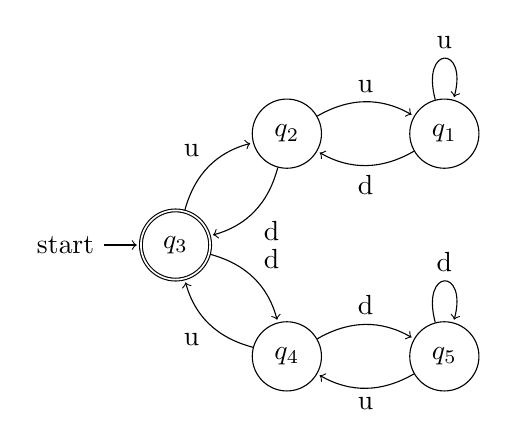
\begin{tikzpicture}[shorten >=1pt,node distance=2cm,on grid,auto]
      \node[state,initial,accepting] (q_3) {$q_3$};
      \node[state] (q_2) [above right=of q_3] {$q_2$};
      \node[state] (q_1) [right=of q_2] {$q_1$};
      \node[state] (q_4) [below right=of q_3] {$q_4$};
      \node[state] (q_5) [right=of q_4] {$q_5$};
        \path[->]
          (q_1) edge [loop above] node {u} ()
                edge [bend left] node {d} (q_2)
          (q_2) edge [bend left] node {u} (q_1)
                edge [bend left] node {d} (q_3)
          (q_3) edge [bend left] node {u} (q_2)
                edge [bend left] node {d} (q_4)
          (q_4) edge [bend left] node {u} (q_3)
                edge [bend left] node {d} (q_5)
          (q_5) edge [bend left] node {u} (q_4)
                edge [loop above] node {d} ();
    \end{tikzpicture}

  \item[1.12:] Regular Expression: $b(bb)^*(aa)^*$
    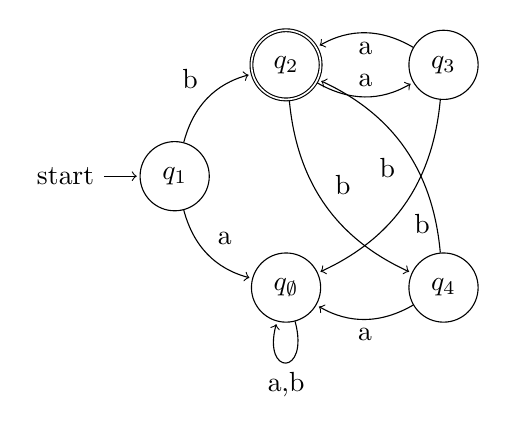
\begin{tikzpicture}[shorten >=1pt,node distance=2cm, on grid,auto]
      \node[state,initial]    (q_1)                             {$q_1$};
      \node[state,accepting]  (q_2)     [above right =of q_1]   {$q_2$};
      \node[state]            (q_3)     [right =of q_2]         {$q_3$};
      \node[state]            (q_null)  [below right =of q_1]   {$q_\emptyset$};
      \node[state]            (q_4)     [right =of q_null]      {$q_4$};
        \path[->]
          (q_1)     edge [bend right] node {a} (q_null)
                    edge [bend left] node {b} (q_2)
          (q_2)     edge [bend right] node {a} (q_3)
                    edge [bend right] node {b} (q_4)
          (q_3)     edge [bend right] node {a} (q_2)
                    edge [bend left] node {b} (q_null)
          (q_4)     edge [bend left] node {a} (q_null)
                    edge [bend right] node {b} (q_2)
          (q_null)  edge [loop below] node {a,b} ();
    \end{tikzpicture}
  \item[1.16.a] (See Diagram Below) \\
        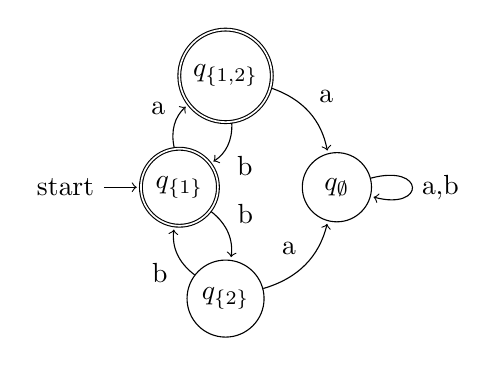
\begin{tikzpicture}[shorten >=1pt,node distance=2cm, on grid,auto]
          \node[state] (q_null) {$q_\emptyset$};
          \node[state,initial,accepting] (q_1) [left=of q_null] {$q_{\{1\}}$};
          \node[state] (q_2) [below left=of q_null] {$q_{\{2\}}$};
          \node[state,accepting] (q_12) [above left=of q_null] {$q_{\{1,2\}}$};
            \path[->]
              (q_null)  edge [loop right] node {a,b} ()
              (q_1)     edge [bend left] node {a} (q_12)
                        edge [bend left] node {b} (q_2)
              (q_2)     edge [bend right] node {a} (q_null)
                        edge [bend left] node {b} (q_1)
              (q_12)    edge [bend left] node {a} (q_null)
                        edge [bend left] node {b} (q_1);
        \end{tikzpicture}

  \item[1.16.b] (See Diagram Below) \\
        \begin{tikzpicture}[shorten >=1pt,node distance=2cm, on grid,auto]
          \node[state,accepting]          (q_2)     [above right =of q_12]  {$q_{\{2\}}$};
          \node[state,initial,accepting]  (q_12)                            {$q_{\{1,2\}}$};
          \node[state]                    (q_13)    [right =of q_12]        {$q_{\{1,3\}}$};
          \node[state,accepting]          (q_23)    [right =of q_13]        {$q_{\{2,3\}}$};
          \node[state]                    (q_null)  [below right =of q_13]        {$q_\emptyset$};
            \path[->]
              (q_2)     edge [bend right] node {a} (q_12)
                        edge [bend right] node {b} (q_null)
              (q_12)    edge [bend right] node {a} (q_13)
                        edge [bend right] node {b} (q_null)
              (q_13)    edge [bend right] node {a} (q_23)
                        edge [bend right] node {b} (q_null)
              (q_23)    edge [bend right] node {a} (q_2)
                        edge [loop right] node {b} ()
              (q_null)  edge [loop right] node {a,b} ();
        \end{tikzpicture}

  \item[1.18.a:] The regular expression for $1.16.a$ is: $a\cup(ab)^*$
  \item[1.18.b:] The regular expression for $1.16.b$ is: $(aab^*)^*$
  \item[1.31:] Suppose a base case where $w$ is a string of length $1$, then $w = w^R$ and thus $A^R$ is regular.
    Now for an induction step, suppose $w = xy$ where $x$ and $y$ are both substrings. Then $w^R = yx$ and $A^R$ is regular via closure of the concatenation operation over the regular language of $x$ and $y$.
  \item[1.41:] A perfect shuffle can be achieved via star composed with the concatenation of $A$ and $B$. If both $A$ and $B$ are regular, then $A \circ B$ is closed as concatenation is a regular operation. And if $A \circ B$ is regular, then $(A \circ B)^*$ is regular as the star operation is also closed over regular languages.
  \item[1.71.a] $A$ is a regular language because we can construct a finite autonoma for it. If for instance, we had $A = \{0^k10^k|k\geq1$ and $u \in \Sigma^*\}$, the language would be irregular due to the lack of a constraint on the upper bound of $k$, as the DFA would have to backtrack $k$ transitions exactly, so the value must be known apriori. However, $u$ can be an unbounded sequence of any combination of $0$ and $1$. Thus, a DFA for $A = \{0^ku0^k|k\geq1$ and $u \in \Sigma^*\}$ can be built that will still handle arbitrarily large values for $k$, because $0^k$ is a valid string in $\Sigma^*$.
  \item[1.71.b] $B$ is not a regular language because we do not have constriants on the size of $k$, thus we need to backtrack $k+1$ states because of the required $1$ following the initial string of $0^k$. However, we cannot backtrack $k+1$ states with just $0^k$. So by the pigeonhole principle, a DFA cannot exist for $B$ and it is non-regular.
\end{itemize}
\end{document}
